\documentclass[conference]{IEEEtran}
\IEEEoverridecommandlockouts
% The preceding line is only needed to identify funding in the first footnote. If that is unneeded, please comment it out.
\usepackage{cite}
\usepackage{amsmath,amssymb,amsfonts}
\usepackage{algorithmic}
\usepackage{graphicx}
\usepackage{textcomp}
\usepackage{xcolor}
\def\BibTeX{{\rm B\kern-.05em{\sc i\kern-.025em b}\kern-.08em
    T\kern-.1667em\lower.7ex\hbox{E}\kern-.125emX}}
\begin{document}

\title{Beat the Quantum Machine - Project Report\\
}

\author{\IEEEauthorblockN{ Team "Beat the Quantum Machine"}
%\IEEEauthorblockA{\textit{dept. name of organization (of Aff.)} \\
%\textit{name of organization (of Aff.)}\\
%City, Country \\email address or ORCID}
%\and
%\IEEEauthorblockN{2\textsuperscript{nd} Given Name Surname}
%\and
%\IEEEauthorblockN{3\textsuperscript{rd} Given Name Surname}
%\and
%\IEEEauthorblockN{4\textsuperscript{th} Given Name Surname}
%\and
%\IEEEauthorblockN{5\textsuperscript{th} Given Name Surname}

}

\maketitle

\begin{abstract}
Games are an interesting test bed for artificial intelligence research, as they provide a self-contained environment with fixed rules. Othello is a perfect information, zero-sum, two-player strategy game played on an $8\times8$ board, and has already been used in classical artificial intelligence research. The board stages are highly volatile, each new move can change a large area of the board. Despite its simple rules, the game of Othello is not trivial, containing of approximately $10^{28}$ legal positions. We propose the implementation of a Quantum Othello game using quantum computing together with classical machine
learning techniques to create a (self-improving) computer opponent players can compete against. Othello is also seen as a Markov Decision Problem in reinforcement learning. The Quantum opponent is designed using a Variational Quantum Circuit for Deep Reinforcement Learning. The implementation utilises PyTorch to train a Deep Q-Learning neural network with a Quantum Computing based hidden layer.
\\ 
\end{abstract}

\begin{IEEEkeywords}
Quantum Machine Learning, Reinforcement Learning, Qiskit
\end{IEEEkeywords}

\section{Introduction}
In recent years, an increasing number of work have been published with the aim of combining the disciplines of quantum information processing and Machine Learning. Theories to merge these two fields have been put forward regularly since quantum information became an independent discipline.
And as we know almost all the games nowadays are based on machine learning, the question that can be asked is why not use this new technique quantum machine learning to develop the games and also in order to be usable in quantum computers because of their efficiency compared to classical computers.
\\ 

\section{Background}

\subsection{Reinforcement Learning}

We don't want to hard-code knowledge about the environment and the best action to take in each case; that would be too much work and would become useless at the slightest change in the environment. We need methods that allow the agent to learn by itself to find the best moves to achieve the best cumulative reward.
Reinforcement learning offers a solution here that differs from supervised and unsupervised learning methods. There are no predefined labels as in supervised learning. However, the reward system also leaves us not completely blind as in unsupervised learning. Rewards can be positive, negative or neutral. While the agent observes the rewards and relates them to the action performed, it can learn how to perform actions better.


The aim of the project was to:
\begin{itemize} 
	\item show feasibility of using Deep Q-Reinforcement Learning powered by Quantum Circuits using a Game setting, and
	\item provide modular Framework for future Quantum ML Tests in an environment with fixed rules for the Quantum Community
\end{itemize}

\subsection{Variational Quantum Circuits And Deep Q-Learning}
Deep Q- Networks is a popular method for computer games. The results in \cite{nature}  marked an important step in reinforcement learning, because it demonstrated that it is possible to use non-linear approximations with this method. This evidence led to a great deal of interest in the field of Q-learning in particular and reinforcement learning in general 

Deep-Q-Learning. Deep reinforcement learning reached a milestone in 2015 when AlphaGo, a computer program trained with deep Reinforcement Learning became the first computer program to beat a human professional Go player on a full-sized $19\times19$ board.
For the game of Othello two Deep-Q-Learning methods are applicable:

\begin{itemize} 
\item  Application of Q-Learning to Grid-World Environments (Tabular Q-Learning),
\item  Q-learning in conjunction with neural networks, a combination referred to as Deep-Q-Network (DQN).
\end{itemize}

The Tabular Q-Learning approach is not practical for large state spaces or a large number of actions. In the case of Othello, there are too many states for this method, which must be recorded and for which approximate values must be calculated.
\\
Deep-Q-Network addresses these difficulties and is therefore used in this approach. 
\\ 
\section{Implementation}
There are many parts in which this project is divided into. Specifically, the game engine is developed by the idea initiator Barbora Hrdá, the classical machine learning is handled by Enda Cahill and Nouhaila Innan, the Quantum Machine learning part is managed by David Peral and Enda Cahill, the usage of Qiskit in this project is handled by Divyanshu Singh and Barbora Hrdá. And last but not the least the documentation and video creation is handled by Barbora Hrdá and Divyanshu Singh. 
We have decided to build on the shoulders of giants and therefore looked for a neural network approach that we can suitably extend with a quantum layer in order to create a hybrid Quantum Classical Neural Network. After a thorough research we decided to use the approach of \cite{a1}., because it used exactly the structure that is suitable for Othello and could be used in Deep Q Reinforcement Learning.  
The most important classes for the game we derived from this are shown in Figure \ref{classes}. 
%``Fig.~\ref{fig}'', even at the beginning of a sentence.


\begin{figure}[htbp]
\centerline{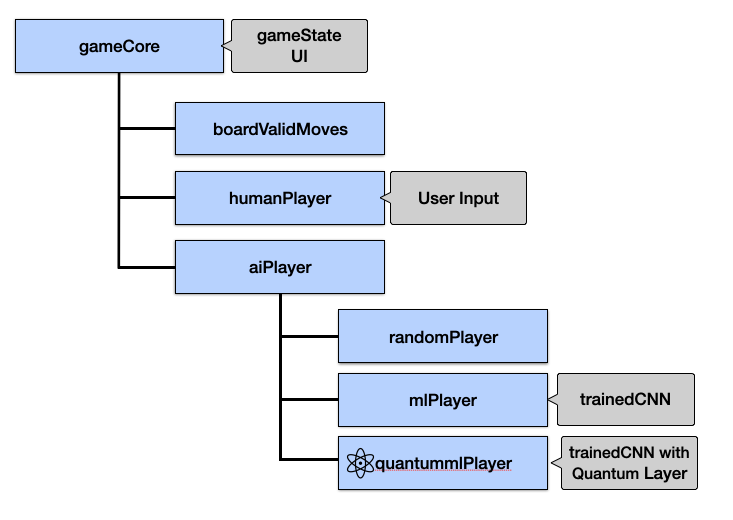
\includegraphics[width=50mm,scale=0.5]{Classes.png}}
\caption{Most important classes for the modular structure.}
\label{classes}
\end{figure}

We wanted to extend this neural network with a quantum layer in order to use the computational power of the quantum computers to speed up the computation on the one hand and to investigate the results that this hybrid quantum network should deliver on the other hand. 
In order to achieve this, we have designed the following layers of the network: 
\\
\begin{itemize} 
\item Input Layer 
\item Convolutional Layer 
\item Fully Connected Layer
\item Quantum Layer
\item Output Layer
\end{itemize}

\subsection{Input Layer}
The input layer receives an 8x8 board converted to torch tensor format. It also recieves information about the current state, the action taken, rewards and evaluates the next state.

\subsection{Convolutional Layer}
The Convolutional layer is used to convolve the input and pass it to the next layer. 

\subsection{Fully Connected Layer}
Recieves the batch normalization of the convolutional layer. It also designed to connect every node in the Convolutional Layer to every node in the Quantum Layer. 

\subsection{Quantum Layer}
In our approach the Quantum Layer recieves 16 outputs which are used to map to the segments of the board to 4 Qubits. A classical approch can then evaluate the allowed moves in that segment. 

\subsection{Output Layer}
The last layer performs optimisation routines and updates parameters, if necessary and returns these values to the game. 
\\ 

These layers are summarized in three parts shown with the used tools for the realisation of the layers in Figure \ref{nodes}. 
\begin{figure}[htbp]
	\centerline{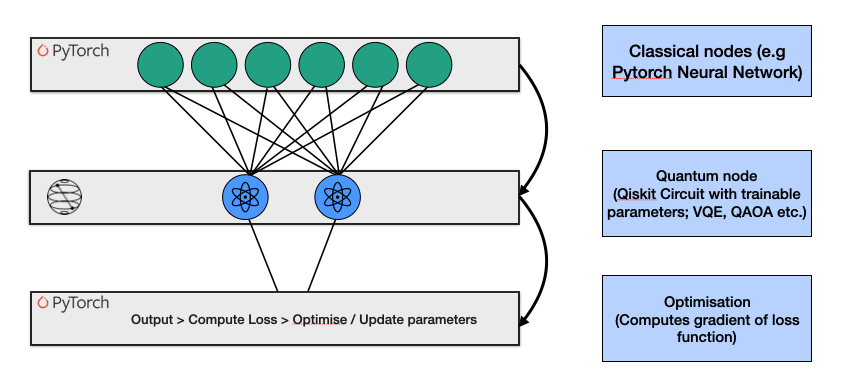
\includegraphics[width=50mm,scale=0.5]{Nodes.png}}
	\caption{Summarized Neural Network Structure.}
	\label{nodes}
\end{figure}

For the classical machine learning modules we used PyTorch, as well as the Torch connector for Qiskit. Using the Machine Learning Library in Qiskit was a advantage in this project, making hybrid neural networks possible. 

\section{Results}
The approach showed that is is possible to start on classical machine learning techniques and combine them with Qiskit. In our approach, we mainly faced the problem of dimension mismatching. The backpropagation of the neural network did not cope with the answers of the quantum layer. Here, a different vector space was returned than the classical network would expect. This problem persists and could not be solved by the end of the project. \\ 


\section{Impact and Further Research}
The value is a project the qiskit community can use in order to try out different hybrid ML approaches in an environment with predefined rules and learning about how to apply these algorithms in different areas other than enhanching game development strategies. 
The general applicability and flexibility of reinforcement learning comes at a price. The biggest obstacle to reinforcement learning in this game setting is that rewards for an action may be delayed considerably. In Othello, as well as in chess, a single strong move in the middle of the game can be game-changing. In learning, we need to recognize such things, which can be difficult when we focus purely on the game play and actions. In future Work the sum of future discounted rewards should be taken more into consideration.
Also, the debugging in novel hybrid approaches, as we describe here, has to be done thoroughly and is therefore time-consuming. At this point, it is definitivly worthwhile to go troubleshooting again to bring the Quantum opponent to life.




%``Fig.~\ref{fig}'', even at the beginning of a sentence.


%\begin{figure}[htbp]
%\centerline{\includegraphics{fig1.png}}
%\caption{Example of a figure caption.}
%\label{fig}
%\end{figure}


\begin{thebibliography}{00}
\bibitem{a1} https://github.com/colinmsnow/othelloAI
\bibitem{a2} https://pytorch.org/tutorials/intermediate/reinforcement\_q\_learning.html
\bibitem{nature} https://www.nature.com/articles/nature14236
\bibitem{b1} Zhifei Zhang and Yuechuan Chen (2014): Searching Algorithms in Playing Othello
\bibitem{b2} Nicolas A. Barriga, Marius Stanescu, Michael Buro (2017): Combining Strategic Learning and Tactical Search in Real-Time Strategy Games In: Proceedings, The Thirteenth AAAI Conference on Artificial Intelligence and Interactive Digital Entertainment (AIIDE-17)
\bibitem{b3} Kory Becker(2019): Flying Unicorn: Developing a Game for a Quantum Computer. In: https://github.com/primaryobjects/flying-unicorn
\bibitem{b4} Paweł Liskowski, Wojciech Jaśkowski, Krzysztof Krawiec (2017): Learning to Play Othello with Deep Neural
Networks. In:IEEE Transactions on Computational Intelligence and AI in Games
\bibitem{b5}: Hlynur Hlynsson (2017): Predicting expert moves in the game of Othello using fully convolutional neural networks
\bibitem{b6}: Samuel Yen-Chi Chen, et al. (2020): Variational Quantum Circuits for Deep Reinforcement Learning
\end{thebibliography}
\vspace{12pt}

\end{document}
